\documentclass[landscape, 10pt]{article}
\usepackage[landscape, margin=0.5in]{geometry}
\usepackage{tikz}
\usetikzlibrary{shapes.geometric, arrows.meta, positioning, fit, backgrounds, matrix, decorations.pathmorphing}

% ─── Colors ───
\definecolor{clrCall}{HTML}{E3F2FD}
\definecolor{clrBook}{HTML}{E8F5E9}
\definecolor{clrGPS}{HTML}{FFF3E0}
\definecolor{clrMBBS}{HTML}{F3E5F5}
\definecolor{clrSpec}{HTML}{E0F7FA}
\definecolor{clrNurse}{HTML}{FCE4EC}
\definecolor{clrNutri}{HTML}{F1F8E9}
\definecolor{clrCare}{HTML}{FFF8E1}
\definecolor{clrDiag}{HTML}{EFEBE9}
\definecolor{clrBill}{HTML}{E8EAF6}
\definecolor{clrNotify}{HTML}{FBE9E7}
\definecolor{clrData}{HTML}{ECEFF1}

% ─── Node Styles ───
\tikzset{
  stage/.style = {rectangle, rounded corners, minimum width=2.9cm, minimum height=1.0cm,
                  align=center, font=\bfseries\footnotesize, draw, thick},
  process/.style = {rectangle, rounded corners, minimum width=2.5cm, minimum height=0.65cm,
                    align=center, font=\scriptsize, draw},
  data/.style = {cylinder, shape border rotate=90, aspect=0.2, minimum width=1.4cm,
                 minimum height=0.55cm, align=center, font=\tiny, draw, fill=clrData},
  arrow/.style = {->, >=Stealth, thick},
  darrow/.style = {->, >=Stealth, thick, dashed, color=blue!60},
  label/.style = {font=\tiny\itshape, text=blue!70},
}

\begin{document}

\pagestyle{empty}

% ══════════════════════════════════════════════════════════════════
% FIGURE 1: HIGH-LEVEL WORKFLOW WITH DATA FLOW
% ══════════════════════════════════════════════════════════════════
\begin{figure}[p]
\centering

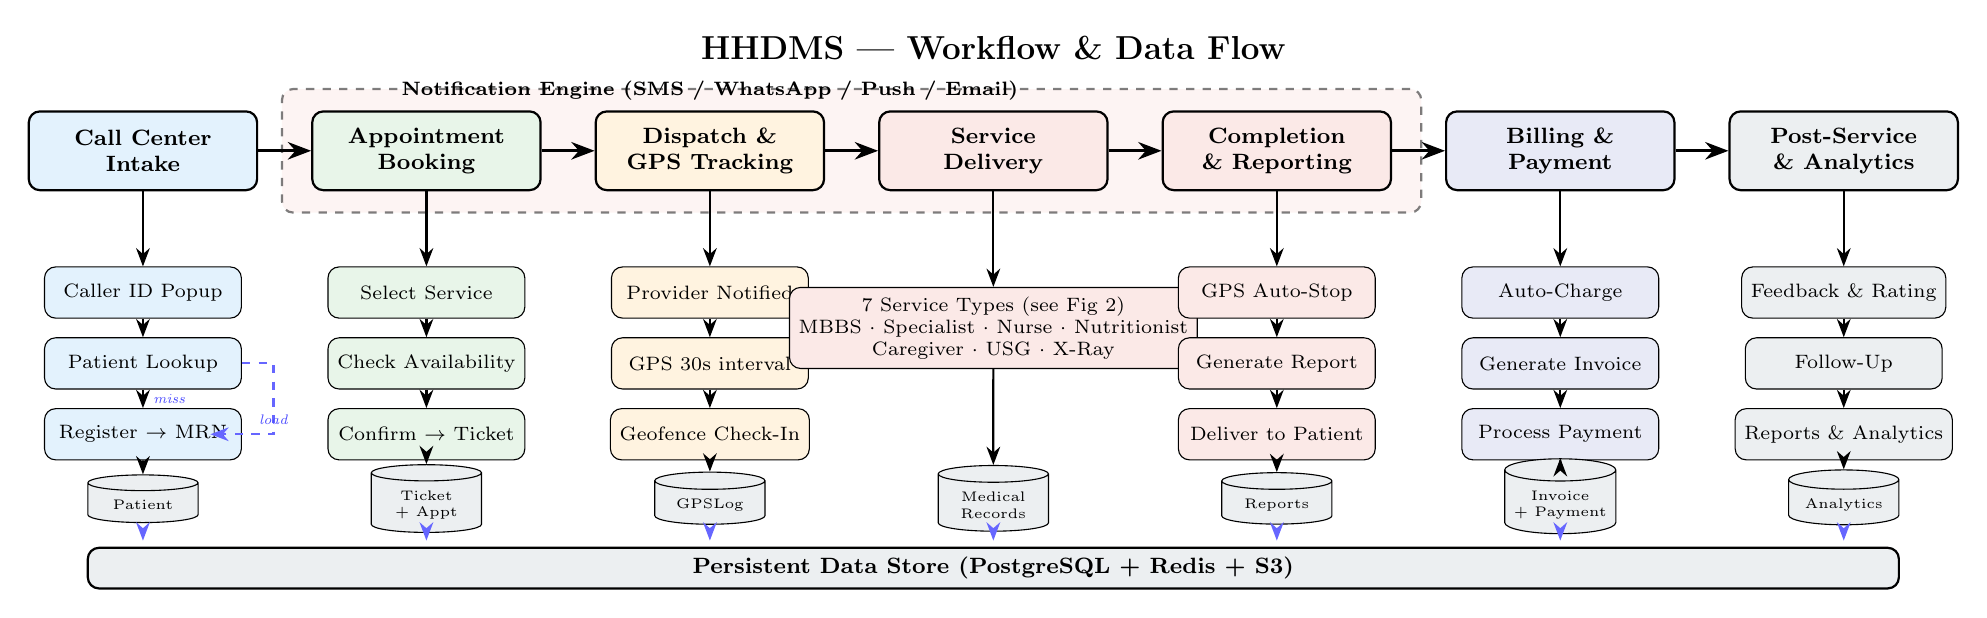
\begin{tikzpicture}
  % x-positions for each column center
  \def\colA{0}
  \def\colB{3.6}
  \def\colC{7.2}
  \def\colD{10.8}
  \def\colE{14.4}
  \def\colF{18.0}
  \def\colG{21.6}
  \def\yStage{0}
  \def\yPOne{-1.8}
  \def\yPTwo{-2.7}
  \def\yPThree{-3.6}
  \def\yData{-4.5}
  \def\yDB{-5.3}

  % --- Stages ---
  \node[stage, fill=clrCall]  at (\colA, \yStage) (S1) {Call Center\\Intake};
  \node[stage, fill=clrBook]  at (\colB, \yStage) (S2) {Appointment\\Booking};
  \node[stage, fill=clrGPS]   at (\colC, \yStage) (S3) {Dispatch \&\\GPS Tracking};
  \node[stage, fill=clrNotify] at (\colD, \yStage) (S4) {Service\\Delivery};
  \node[stage, fill=clrNotify] at (\colE, \yStage) (S5) {Completion\\\& Reporting};
  \node[stage, fill=clrBill]  at (\colF, \yStage) (S6) {Billing \&\\Payment};
  \node[stage, fill=clrData]  at (\colG, \yStage) (S7) {Post-Service\\\& Analytics};

  % Stage links
  \draw[arrow, very thick] (S1.east) -- (S2.west);
  \draw[arrow, very thick] (S2.east) -- (S3.west);
  \draw[arrow, very thick] (S3.east) -- (S4.west);
  \draw[arrow, very thick] (S4.east) -- (S5.west);
  \draw[arrow, very thick] (S5.east) -- (S6.west);
  \draw[arrow, very thick] (S6.east) -- (S7.west);

  % --- Process nodes ---
  % Col 1
  \node[process, fill=clrCall]  at (\colA, \yPOne)   (P1a) {Caller ID Popup};
  \node[process, fill=clrCall]  at (\colA, \yPTwo)   (P1b) {Patient Lookup};
  \node[process, fill=clrCall]  at (\colA, \yPThree) (P1c) {Register $\to$ MRN};
  \draw[arrow] (S1.south) -- (P1a.north);
  \draw[arrow] (P1a.south) -- (P1b.north);
  \draw[arrow] (P1b.south) -- node[right, label] {miss} (P1c.north);
  \draw[darrow] (P1b.east) -- ++(0.4,0) |- ([xshift=-0.4cm] P1c.east)
    node[pos=0.4, label] {load};

  % Col 2
  \node[process, fill=clrBook]  at (\colB, \yPOne)   (P2a) {Select Service};
  \node[process, fill=clrBook]  at (\colB, \yPTwo)   (P2b) {Check Availability};
  \node[process, fill=clrBook]  at (\colB, \yPThree) (P2c) {Confirm $\to$ Ticket};
  \draw[arrow] (S2.south) -- (P2a.north);
  \draw[arrow] (P2a.south) -- (P2b.north);
  \draw[arrow] (P2b.south) -- (P2c.north);

  % Col 3
  \node[process, fill=clrGPS]   at (\colC, \yPOne)   (P3a) {Provider Notified};
  \node[process, fill=clrGPS]   at (\colC, \yPTwo)   (P3b) {GPS 30s interval};
  \node[process, fill=clrGPS]   at (\colC, \yPThree) (P3c) {Geofence Check-In};
  \draw[arrow] (S3.south) -- (P3a.north);
  \draw[arrow] (P3a.south) -- (P3b.north);
  \draw[arrow] (P3b.south) -- (P3c.north);

  % Col 4 — wider box for service types
  \node[process, fill=clrNotify, minimum width=4.5cm]
    at (\colD, -2.25) (P4) {7 Service Types (see Fig 2)\\
    MBBS $\cdot$ Specialist $\cdot$ Nurse $\cdot$ Nutritionist\\
    Caregiver $\cdot$ USG $\cdot$ X-Ray};
  \draw[arrow] (S4.south) -- (P4.north);

  % Col 5
  \node[process, fill=clrNotify] at (\colE, \yPOne)   (P5a) {GPS Auto-Stop};
  \node[process, fill=clrNotify] at (\colE, \yPTwo)   (P5b) {Generate Report};
  \node[process, fill=clrNotify] at (\colE, \yPThree) (P5c) {Deliver to Patient};
  \draw[arrow] (S5.south) -- (P5a.north);
  \draw[arrow] (P5a.south) -- (P5b.north);
  \draw[arrow] (P5b.south) -- (P5c.north);

  % Col 6
  \node[process, fill=clrBill]  at (\colF, \yPOne)   (P6a) {Auto-Charge};
  \node[process, fill=clrBill]  at (\colF, \yPTwo)   (P6b) {Generate Invoice};
  \node[process, fill=clrBill]  at (\colF, \yPThree) (P6c) {Process Payment};
  \draw[arrow] (S6.south) -- (P6a.north);
  \draw[arrow] (P6a.south) -- (P6b.north);
  \draw[arrow] (P6b.south) -- (P6c.north);

  % Col 7
  \node[process, fill=clrData]  at (\colG, \yPOne)   (P7a) {Feedback \& Rating};
  \node[process, fill=clrData]  at (\colG, \yPTwo)   (P7b) {Follow-Up};
  \node[process, fill=clrData]  at (\colG, \yPThree) (P7c) {Reports \& Analytics};
  \draw[arrow] (S7.south) -- (P7a.north);
  \draw[arrow] (P7a.south) -- (P7b.north);
  \draw[arrow] (P7b.south) -- (P7c.north);

  % --- Data nodes ---
  \node[data] at (\colA, \yData) (D1) {Patient};
  \node[data] at (\colB, \yData) (D2) {Ticket\\+ Appt};
  \node[data] at (\colC, \yData) (D3) {GPSLog};
  \node[data] at (\colD, \yData) (D4) {Medical\\Records};
  \node[data] at (\colE, \yData) (D5) {Reports};
  \node[data] at (\colF, \yData) (D6) {Invoice\\+ Payment};
  \node[data] at (\colG, \yData) (D7) {Analytics};

  \draw[arrow] (P1c.south) -- (D1.north);
  \draw[arrow] (P2c.south) -- (D2.north);
  \draw[arrow] (P3c.south) -- (D3.north);
  \draw[arrow] (P4.south) -- (D4.north);
  \draw[arrow] (P5c.south) -- (D5.north);
  \draw[arrow] (P6c.south) -- (D6.north);
  \draw[arrow] (P7c.south) -- (D7.north);

  % --- Notification Engine label at top (does NOT overlay process/data) ---
  \begin{scope}[on background layer]
    \coordinate (NE1) at ([xshift=-0.3cm, yshift=0.2cm] S2.north west);
    \coordinate (NE2) at ([xshift=0.3cm, yshift=-0.2cm] S5.south east);
    \node[fill=clrNotify, draw, thick, rounded corners, dashed, opacity=0.5,
          fit={(NE1) (NE2)}, inner sep=2pt] {};
    \node[font=\scriptsize\bfseries, above] at (S3.north)
      {Notification Engine (SMS / WhatsApp / Push / Email)};
  \end{scope}

  % --- Common database bar at bottom ---
  \node[fill=clrData, draw, thick, rounded corners, minimum width=23cm, minimum height=0.4cm,
        font=\footnotesize\bfseries, align=center] at (10.8, \yDB) (DB) {Persistent Data Store (PostgreSQL + Redis + S3)};

  % Data flow arrows down to DB
  \foreach \col in {0,3.6,7.2,10.8,14.4,18.0,21.6} {
    \draw[darrow] (\col, \yData-0.3) -- (\col, \yDB+0.35);
  }

  % Title
  \node[font=\bfseries\large] at (10.8, 1.3) {HHDMS — Workflow \& Data Flow};
\end{tikzpicture}
\caption{High-Level Workflow \& Data Flow}
\end{figure}

% ══════════════════════════════════════════════════════════════════
% FIGURE 2: DETAILED SERVICE DELIVERY FLOW
% ══════════════════════════════════════════════════════════════════
\begin{figure}[p]
\centering
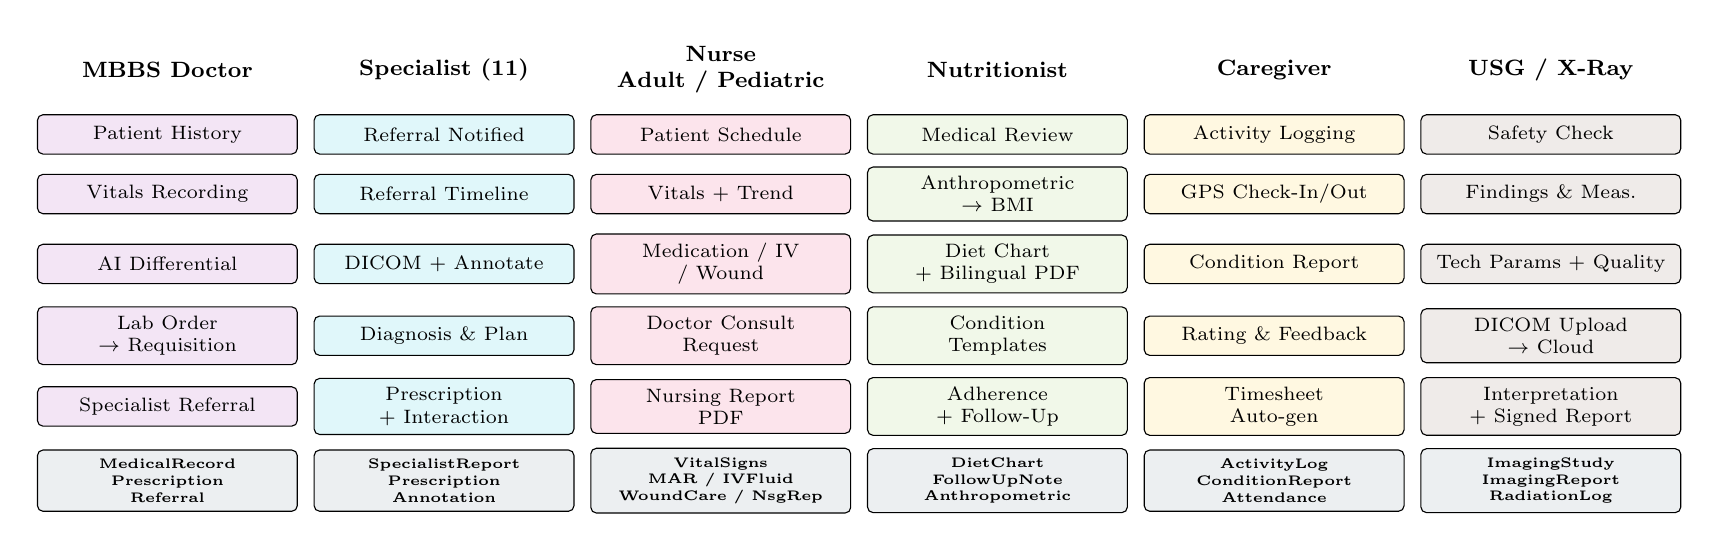
\begin{tikzpicture}[
  box/.style = {rectangle, rounded corners=2pt, minimum width=3.3cm, minimum height=0.5cm,
                align=center, font=\scriptsize, draw, fill=#1},
  entity/.style = {rectangle, rounded corners=2pt, minimum width=3.3cm, minimum height=0.5cm,
                   align=center, font=\tiny, draw, fill=clrData},
  heading/.style = {font=\bfseries\footnotesize, align=center},
]

\matrix[row sep=0.15cm, column sep=0.2cm] {
  % Header
  \node[heading] {MBBS Doctor}; &
  \node[heading] {Specialist (11)}; &
  \node[heading] {Nurse\\Adult / Pediatric}; &
  \node[heading] {Nutritionist}; &
  \node[heading] {Caregiver}; &
  \node[heading] {USG / X-Ray}; \\

  % Row 1
  \node[box=clrMBBS]  {Patient History}; &
  \node[box=clrSpec]  {Referral Notified}; &
  \node[box=clrNurse] {Patient Schedule}; &
  \node[box=clrNutri] {Medical Review}; &
  \node[box=clrCare]  {Activity Logging}; &
  \node[box=clrDiag]  {Safety Check}; \\

  % Row 2
  \node[box=clrMBBS]  {Vitals Recording}; &
  \node[box=clrSpec]  {Referral Timeline}; &
  \node[box=clrNurse] {Vitals + Trend}; &
  \node[box=clrNutri] {Anthropometric\\$\to$ BMI}; &
  \node[box=clrCare]  {GPS Check-In/Out}; &
  \node[box=clrDiag]  {Findings \& Meas.}; \\

  % Row 3
  \node[box=clrMBBS]  {AI Differential}; &
  \node[box=clrSpec]  {DICOM + Annotate}; &
  \node[box=clrNurse] {Medication / IV\\/ Wound}; &
  \node[box=clrNutri] {Diet Chart\\+ Bilingual PDF}; &
  \node[box=clrCare]  {Condition Report}; &
  \node[box=clrDiag]  {Tech Params + Quality}; \\

  % Row 4
  \node[box=clrMBBS]  {Lab Order\\$\to$ Requisition}; &
  \node[box=clrSpec]  {Diagnosis \& Plan}; &
  \node[box=clrNurse] {Doctor Consult\\Request}; &
  \node[box=clrNutri] {Condition\\Templates}; &
  \node[box=clrCare]  {Rating \& Feedback}; &
  \node[box=clrDiag]  {DICOM Upload\\$\to$ Cloud}; \\

  % Row 5
  \node[box=clrMBBS]  {Specialist Referral}; &
  \node[box=clrSpec]  {Prescription\\+ Interaction}; &
  \node[box=clrNurse] {Nursing Report\\PDF}; &
  \node[box=clrNutri] {Adherence\\+ Follow-Up}; &
  \node[box=clrCare]  {Timesheet\\Auto-gen}; &
  \node[box=clrDiag]  {Interpretation\\+ Signed Report}; \\

  % Row 6: bold entity names
  \node[entity] {\textbf{MedicalRecord}\\\textbf{Prescription}\\\textbf{Referral}}; &
  \node[entity] {\textbf{SpecialistReport}\\\textbf{Prescription}\\\textbf{Annotation}}; &
  \node[entity] {\textbf{VitalSigns}\\\textbf{MAR / IVFluid}\\\textbf{WoundCare / NsgRep}}; &
  \node[entity] {\textbf{DietChart}\\\textbf{FollowUpNote}\\\textbf{Anthropometric}}; &
  \node[entity] {\textbf{ActivityLog}\\\textbf{ConditionReport}\\\textbf{Attendance}}; &
  \node[entity] {\textbf{ImagingStudy}\\\textbf{ImagingReport}\\\textbf{RadiationLog}}; \\
};
\end{tikzpicture}
\caption{Detailed Service Delivery — Per-Type Workflow \& Data Entities Written}
\end{figure}

% ══════════════════════════════════════════════════════════════════
% FIGURE 3: DATA ENTITY RELATIONSHIP DIAGRAM
% ══════════════════════════════════════════════════════════════════
\begin{figure}[p]
\centering
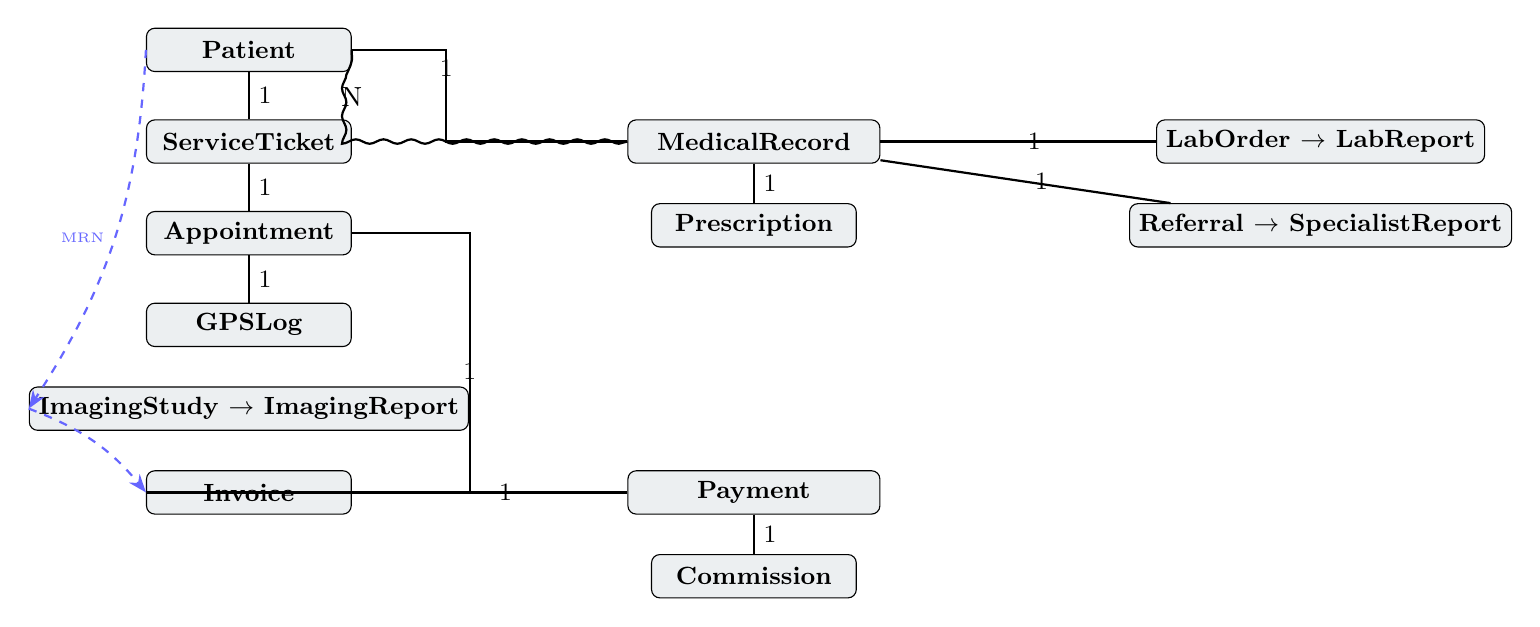
\begin{tikzpicture}[
  ent/.style = {rectangle, rounded corners=3pt, minimum width=2.6cm, minimum height=0.55cm,
                align=center, font=\small\bfseries, draw, fill=clrData},
  ent2/.style = {rectangle, rounded corners=3pt, minimum width=3.2cm, minimum height=0.55cm,
                 align=center, font=\small\bfseries, draw, fill=clrData},
  rel/.style = {thick},
  one/.style = {rel, node font=\small},
  many/.style = {rel, decorate, decoration={snake, amplitude=0.8pt}},
]

  % Vertical spine: Patient -> Ticket -> Appointment -> GPSLog
  \node[ent]  (Patient) {Patient};
  \node[ent, below=0.6cm of Patient] (Ticket)  {ServiceTicket};
  \node[ent, below=0.6cm of Ticket]  (Appt)    {Appointment};
  \node[ent, below=0.6cm of Appt]    (GPS)     {GPSLog};

  % Upper right: MedicalRecord, Prescription
  \node[ent2, right=3.5cm of Ticket] (MedRec)  {MedicalRecord};
  \node[ent,  below=0.5cm of MedRec] (RX)      {Prescription};

  % Further right: Lab, Referral
  \node[ent2, right=3.5cm of MedRec] (Lab)     {LabOrder $\to$ LabReport};
  \node[ent2, below=0.5cm of Lab]    (Refer)   {Referral $\to$ SpecialistReport};

  % Lower left: Imaging, Invoice, Payment, Commission
  \node[ent2, below=0.5cm of GPS]    (Image)   {ImagingStudy $\to$ ImagingReport};
  \node[ent,  below=0.5cm of Image]  (Invoice) {Invoice};
  \node[ent2, right=3.5cm of Invoice](Payment) {Payment};
  \node[ent,  below=0.5cm of Payment](Comm)    {Commission};

  % Relationships (1:N)
  \draw[one]  (Patient)  -- node[right] {1} (Ticket);
  \draw[one]  (Ticket)   -- node[right] {1} (Appt);
  \draw[one]  (Appt)     -- node[right] {1} (GPS);

  % Patient 1 --- N MedicalRecord
  \draw[one]  (Patient.east) -- ++(1.2,0) |- node[pos=0.2, above] {1} (MedRec.west);
  \draw[many] (MedRec.west)  -| node[pos=0.85, below] {N} (Patient.east);

  \draw[one]  (MedRec) -- node[right] {1} (RX);
  \draw[one]  (MedRec) -- node[right] {1} (Lab);
  \draw[one]  (MedRec) -- node[right] {1} (Refer);

  % Billing
  \draw[one]  (Appt.east) -- ++(1.5,0) |- node[pos=0.3, above] {1} (Invoice.west);
  \draw[one]  (Invoice) -- node[right] {1} (Payment);
  \draw[one]  (Payment) -- node[right] {1} (Comm);

  % Cross-links via MRN
  \draw[darrow, bend left=15] (Patient.west) to node[left, font=\tiny] {MRN} (Image.west);
  \draw[darrow, bend left=15] (Image.west) to (Invoice.west);

\end{tikzpicture}
\caption{Core Data Entity Relationships (1:N cardinality)}
\end{figure}

\end{document}
